\apendice{Especificación de Requisitos}

\section{Introducción}
Este segundo apéndice recuerda los objetivos generales marcados en el proyecto, y que previamente se han comentado en la memoria. Además tratará el catálogo de requisitos junto con su especificación y diagramas de caso de uso.

\section{Objetivos generales}
El proyecto se ha maracdo los siguientes objetivos generales:
\begin{itemize}
    \item Ayudar a la empresa que origina el proyecto, consiguiendo que se puedan identificar el mayor número de bobinas con errores aprovechables por parte de la empresa.
    \item Aumentar la eficiencia de la cadena de galvanizado de la empresa, de manera que un operario no tenga que analizar de forma exhaustiva cada bobina, para saber si es utilizable o no.
    \item Crear una cadena más sostenible, consiguiendo que se puedan aprovechar al máximo las bobinas galvanizadas y evitar que se tenga que desperdiciar demasiado material.   
\end{itemize}

\section{Catalogo de requisitos}
A continuación se indican los requisitos marcados en la aplicación llevada a cabo en el proyecto:
\begin{itemize}
    \item \textbf{REQ 1:} conseguir una aplicación capaz de ejecutar un conjunto de modelos sobre los datos de una bobina.
    \begin{itemize}
        \item \textbf{REQ 1.1:} cargar los datos medidos por los sensores.
        \item \textbf{REQ 1.2:} obtener las principales características de las bobinas.
        \item \textbf{REQ 1.3:} evaluar las bobinas con los modelos.
        \item \textbf{REQ 1.4:} mostrar si la bobina es válida o no.
    \end{itemize}
     \item \textbf{REQ 2:} permitir que los resultados obtenidos puedan descargarse.
    \begin{itemize}
        \item \textbf{REQ 2.1:} descargar las características obtenidas de las bobinas.
        \item \textbf{REQ 2.2:} descargar los rsultados obtenidos por el modelo.
    \end{itemize}
    \item \textbf{REQ 3:} generar un archivo que contenga el historial de las diferentes bobinas cargadas y evaluadas.
        \begin{itemize}
            \item \textbf{REQ 3.1:} guardar en el fichero el día en que se cargó la bobina, junto con la clase predicha.
        \end{itemize}
\end{itemize}

\section{Especificación de requisitos}
\subsection{Actores}
En esta aplicación tan solo se detecta un actor: el operario de la empresa. Ya que es el encargado, una vez se cuenten con los datos obtenidos por los sensores sobre la bobina, de dirigirse a la aplicación y realizar la predicción sobre los mismos.

\newpage
\subsection{Diagrama de casos de uso}
La Figura \ref{f:casus} muestra el diagrama de casos de uso de la aplicación.

\begin{figure}[h]
 \centering
  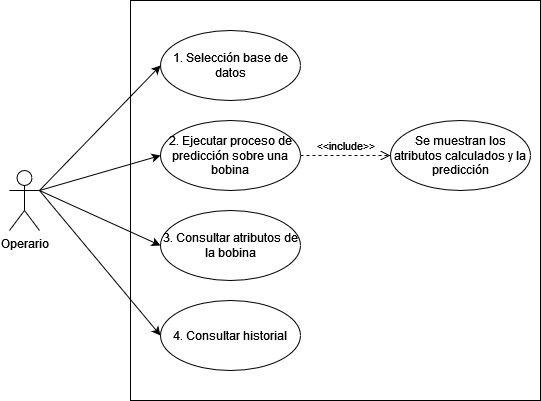
\includegraphics[width=1\textwidth]{img/casosUso.png}
 \caption{Diagrama de Casos de Uso}
 \label{f:casus}
\end{figure}

\newpage
\subsection{Especificación de casos de uso}
A continaucón se muestra una tabla para cada caso de uso:

\begin{center}
\begin{tabular}{|ll|}
\hline
\multicolumn{2}{|l|}{\textbf{CU 1 - Selección base de datos}}                                                                                                                                                          \\ \hline
\multicolumn{1}{|l|}{\textbf{Descripción}}     & \begin{tabular}[c]{@{}l@{}}Permite al operario seleccionar los diferentes valores que \\ permitan conectarse a la base de datos para cargar los valores.\end{tabular} \\ \hline
\multicolumn{1}{|l|}{\textbf{Requisitos}}      & REQ 1.1                                                                                                                                                               \\ \hline
\multicolumn{1}{|l|}{\textbf{Precondiciones}}  & Se está ejecutando el notebook de la aplicación.                                                                                                                      \\ \hline
\multicolumn{1}{|l|}{\textbf{Secuencia}}       & \begin{tabular}[c]{@{}l@{}}1. El usuario rellena los campos: user, password, host y \\ database \\ 2. El usuario ejecuta la celda correspondiente\end{tabular}            \\ \hline
\multicolumn{1}{|l|}{\textbf{Postcondiciones}} & La celda se ejecuta bien y aparece un 2 a su izquierda                                                                                                                \\ \hline
\multicolumn{1}{|l|}{\textbf{Excepciones}}     & \begin{tabular}[c]{@{}l@{}}Se introducen los valores de forma incorrecta y sin el formato \\ necesario en Python y salta un error\end{tabular}                        \\ \hline
\end{tabular}
\captionof{table}{Caso de Uso - 1}
\label{t:caso1}
\end{center}

\begin{center}
\begin{tabular}{|ll|}
\hline
\multicolumn{2}{|l|}{\textbf{CU 2 - Ejecución proceso de predicción sobre una bobina}}                                                                                                                                                                                                                                \\ \hline
\multicolumn{1}{|l|}{\textbf{Descripción}}     & \begin{tabular}[c]{@{}l@{}}Permite al operario seleccionar la ID de la bobina desea\\ sobre la que calcular las predicciones.\end{tabular}                                                                                                                           \\ \hline
\multicolumn{1}{|l|}{\textbf{Requisitos}}      & REQ 1.2, REQ 1.3 y REQ 1.4                                                                                                                                                                                                                                           \\ \hline
\multicolumn{1}{|l|}{\textbf{Precondiciones}}  & \begin{tabular}[c]{@{}l@{}}Se está ejecutando el notebook de la aplicación, y se\\ ha indicado la base de datos.\end{tabular}                                                                                                                                        \\ \hline
\multicolumn{1}{|l|}{\textbf{Secuencia}}       & \begin{tabular}[c]{@{}l@{}}1. El usuario ejecuta la tercera celda.\\ 2. El usuario selecciona en el desplegable la ID de la\\ bobina.\\ 3. El usuario observa los valores y predicciones mostradas\\ por pantalla, y decide si seleccionar otra bobina.\end{tabular} \\ \hline
\multicolumn{1}{|l|}{\textbf{Postcondiciones}} & \begin{tabular}[c]{@{}l@{}}Se muestran los atributos calculados de la bobina y \\ la decisión del modelo.\end{tabular}                                                                                                                                               \\ \hline
\multicolumn{1}{|l|}{\textbf{Excepciones}}     & \begin{tabular}[c]{@{}l@{}}Se produce algún problema durante el proceso y el \\ modelo devuelve algún error.\end{tabular}                                                                                                                                            \\ \hline
\end{tabular}
\captionof{table}{Caso de Uso - 2}
\label{t:caso2}
\end{center}

\begin{center}
\begin{tabular}{|ll|}
\hline
\multicolumn{2}{|l|}{\textbf{CU 3 - Consultar atributos de la bobina}}                                                                                                                                                                                                                  \\ \hline
\multicolumn{1}{|l|}{\textbf{Descripción}}     & \begin{tabular}[c]{@{}l@{}}Permite al operario conocer los atributos y el mapa\\ codificado de la bobina previamente calculados.\end{tabular}                                                                                          \\ \hline
\multicolumn{1}{|l|}{\textbf{Requisitos}}      & REQ 2.1                                                                                                                                                                                                                                \\ \hline
\multicolumn{1}{|l|}{\textbf{Precondiciones}}  & Se ha realizado una predicción sobre la bobina deseada.                                                                                                                                                                                \\ \hline
\multicolumn{1}{|l|}{\textbf{Secuencia}}       & \begin{tabular}[c]{@{}l@{}}1. El usuario se dirige a la ruta donde se encuentra\\ la aplicación.\\ \\ 2. El usuario se dirige al directorio /bobinas.\\ 3. El usuario abre el CSV correspondiente a la \\ bobina deseada.\end{tabular} \\ \hline
\multicolumn{1}{|l|}{\textbf{Postcondiciones}} & \begin{tabular}[c]{@{}l@{}}El usuario consigue abrir el fichero correctamente, y\\ en su interior se encuentran todos los atributos.\end{tabular}                                                                                      \\ \hline
\multicolumn{1}{|l|}{\textbf{Excepciones}}     & -                                                                                                                                                                                                                                      \\ \hline
\end{tabular}
\captionof{table}{Caso de Uso - 3}
\label{t:caso3}
\end{center}

\begin{center}
\begin{tabular}{|ll|}
\hline
\multicolumn{2}{|l|}{\textbf{CU 4 - Consultar el historial}}                                                                                                                                                  \\ \hline
\multicolumn{1}{|l|}{\textbf{Descripción}}     & \begin{tabular}[c]{@{}l@{}}Permite al operario poder revisar el historial de las\\ diferentes predicciones realizadas.\end{tabular}                          \\ \hline
\multicolumn{1}{|l|}{\textbf{Requisitos}}      & REQ 2.2 y REQ 3                                                                                                                                              \\ \hline
\multicolumn{1}{|l|}{\textbf{Precondiciones}}  & \begin{tabular}[c]{@{}l@{}}Se ha realizado al menos una predicción sobre\\ cualquier bobina.\end{tabular}                                                    \\ \hline
\multicolumn{1}{|l|}{\textbf{Secuencia}}       & \begin{tabular}[c]{@{}l@{}}1. El usuario se dirige a la ruta donde se encuentra\\ la aplicación.\\ 2. El usuario sabre el archivo historial.txt\end{tabular} \\ \hline
\multicolumn{1}{|l|}{\textbf{Postcondiciones}} & \begin{tabular}[c]{@{}l@{}}El archivo contiene en su interior los resultados\\ previamente calculados.\end{tabular}                                          \\ \hline
\multicolumn{1}{|l|}{\textbf{Excepciones}}     & -                                                                                                                                                            \\ \hline
\end{tabular}
\captionof{table}{Caso de Uso - 4}
\label{t:caso4}
\end{center}